\newpage
\section{Prinsipiell løsning}
\label{prinsipiellLoesning}

Et anti-aliasing filter brukes for å minske aliasing når man konverter signalet fra et analogt til digitalt signal. Nyquist raten sier at samplingsfrekvensen må være minst dobbelt så høy som den høyeste frekvensen i signalet, for å kunne rekonstruere signalet etter konvertering. De Ideele egenskapene til et anti aliasing filter er at amplituderesopnsen er flat i passbåndet, og at den har en bratt overgang fra passbåndet til stoppbåndet. Jo, brattere overgangen er, jo bedre er filteret. Et anti-aliasing filter realiseres derfor med et veldig agresivt lavpassfilter. Et Butterworth filter vil ha bratt nok overgang til å tilfredstille kravene til et anti-aliasing filter uten å påvirke signalet for mye i passbåndet i motsetning til et Chebyshev filter som skaper ripples i passbåndet.

\subsection{Butterworth filter}
\label{ButterworthFilter}

Et Butterworth filter er et aktivt filter som kun benytter seg av kondensatorer som frekvensavhengige komponenter. Kretstopologien er basert på Sallen-Key filteret som er vist i figur \ref{fig:SallenKey}. Sallen-Key filteret er et aktivt filter som bruker to operasjonsforsterkere, to kondensatorer og to motstander. Filteret kan realisere et andre ordens lavpassfilter med en Butterworth karakteristikk. Kretsen er vist i figur \ref{fig:SallenKey}. 

\begin{figure} [!h]
\centering
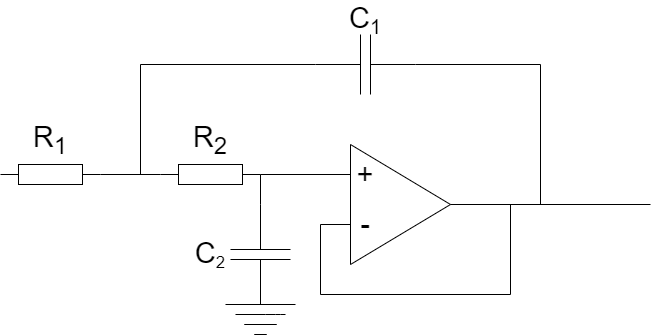
\includegraphics[width=0.7\linewidth]{Bilder/SallenKey.drawio.png}
\caption{Sallen-Key filteret}
\label{fig:SallenKey}
\end{figure}

